\begin{figure}[H]
	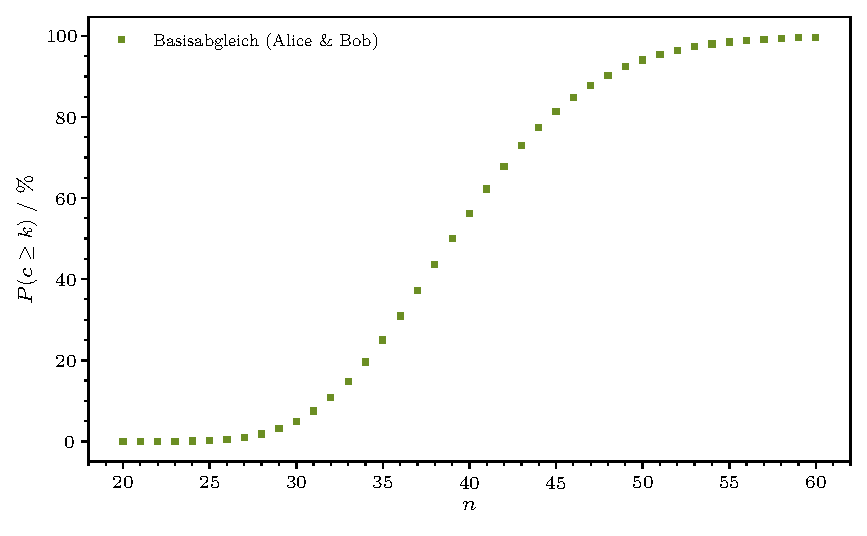
\includegraphics{build/kumuliert.pdf}
	\vspace{-1.5\baselineskip}
	\caption{Kumulierte Wahrscheinlichkeit für das Auftreten von mindestens $k = 20$ passenden Basispaaren in $n$ Messungen
			 zur Schlüsselgeneration.}
	\label{fig:kumuliert}
	\vspace{-2.5\baselineskip}
\end{figure}

\section{Auswertung}

Als Serie gleichartiger und unabhängiger Events lassen sich die Wahrscheinlichkeiten für das Eintreten der verschiedenen
Fälle in diesem Versuch mithilfe der Binomialverteilung
\begin{equation*}
	P(c = k) = f(k, n, p) = \pfrac{n!}{k!(n - k)!} \, p^k (1 - p)^{n - k}
\end{equation*}
bestimmen. Daraus folgt auch die in Abbildung \ref{fig:kumuliert} aufgetragene kumulierte Verteilung
\begin{equation*}
	P(c \geq k) = F(k, n, p) = \!\! \sum_{m \, = \, k}^n \! f(m, n, p)
\end{equation*}
für das Auftreten von $k$ oder mehr Ereignissen mit Einzelwahrscheinlichkeit $p$ aus den insgesamt $n$ diskreten Messungen.
Das zufällige Eintreten gleicher Basen hat $p = \qty{50}{\percent}$~und tritt bei den empfohlenen $n = 52$ Signalen in
\qty{96.48}{\percent} der Fälle ausreichend oft für die geforderte Schlüssellänge $k = 20$ auf.



\subsection{Verschlüsselung einer Nachricht}

\begin{longtable}[c]{rccrcc}
	\caption{.}
	\label{tab:schluessel}
	\\
	\expandableinput{content/tabelle/schluessel.tex}
\end{longtable}

\qty{7.84}{\percent}

\begin{table}[H]
	\centering
	\caption{.}
	\label{tab:alice}
	\begin{tabular}{lcccc}
		\expandableinput{content/tabelle/alice.tex}
	\end{tabular}
\end{table}

\begin{table}[H]
	\centering
	\caption{.}
	\label{tab:bob}
	\begin{tabular}{lcccc}
		\expandableinput{content/tabelle/bob.tex}
	\end{tabular}
\end{table}

\subsection{Identifikation eines Abhörversuchs}

\begin{longtable}[c]{rccrccc}
	\caption{.}
	\label{tab:abhoeren}
	\\
	\expandableinput{content/tabelle/abhoeren.tex}
\end{longtable}

\begin{figure}[H]
	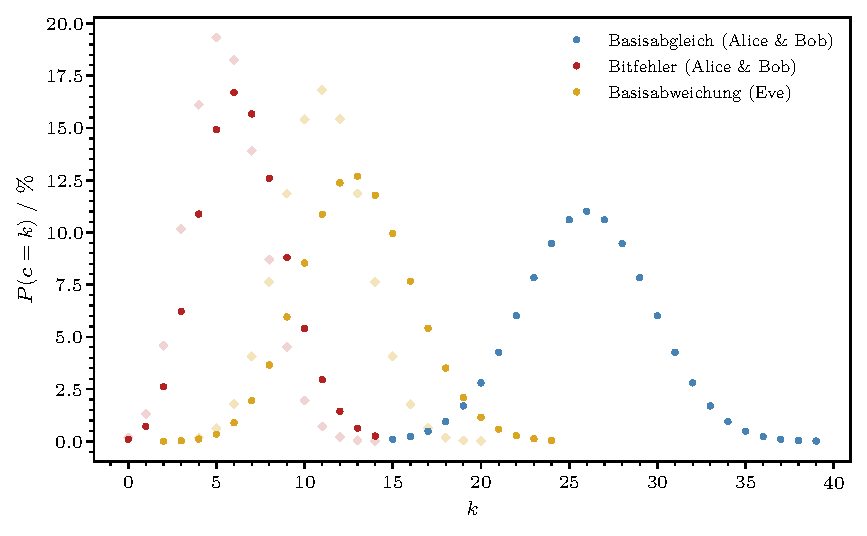
\includegraphics{build/verteilung.pdf}
	\caption{.}
	\label{fig:verteilung}
\end{figure}

\qty{6.01}{\percent}

\qty{10.86}{\percent}

\qty{10.88}{\percent}

\qty{16.82}{\percent}

\qty{16.11}{\percent}
